\documentclass{article}

\usepackage{color}
\usepackage{amsmath}
\usepackage{graphicx}
\usepackage{fullpage}


\sloppy
\definecolor{lightgray}{gray}{0.5}
\setlength{\parindent}{0pt}
\renewcommand{\arraystretch}{1.2}

\newcommand{\tab}{\hspace{20 mm}}

% part numbering command
\newcounter{partNum}
\newcommand{\partNum}{%
        \stepcounter{partNum}%
        \thepartNum}
\newcommand{\sectPart}[1]{\section*{Part \partNum: #1}}

\newcommand{\bitem}[1]{\item \textbf{#1}}

\newcommand{\assignment}{Lab 11}
\newcommand{\duedate}{May 9, 2014}
\newcommand{\header}{\noindent \textbf{ECE348 \assignment, Spring 2014 \\
                     Group C1 \\ 
                     Connor Brem (cbrem) \\
                     Spencer Barton (sebarton) \\
                     \duedate} \vspace{0.10in} \hrule}

\begin{document}
    
%=======================================================

\header

%=======================================================

\begin{center}
    \vspace{1em}
    \Large{MyTOS. YourTOS.} \\
    
\includegraphics[scale=0.25]{../../logo.png}
\end{center}

%-------------------------------------------------------

\sectPart{Coding}

All done.

%-------------------------------------------------------

\sectPart{Code to State-Chart}

%-------------------------------------------------------

\sectPart{Wiring}

%-------------------------------------------------------

\sectPart{Code Review}

    \begin{tabular}{| l | l | l | p{25em} |}
        \hline
        \textbf{Defect \#} & \textbf{File} & \textbf{Line \#} & \textbf{Description} \\ \hline
        1 & OurTOS.c & 111 & Typo. Was \texttt{\_started}. Should be \texttt{!\_started}. \\ \hline
        2 & OurTOS.c & 115 & Interrupt does not run b/c no time between EnableInterrupts and DisableInterrupts. \\ \hline
        3  & OurTOS.c & 132 & Not storing priority in \texttt{task\_t}. \\ \hline
        4 & OurTOS.c & 283 & Should only updates a task's \texttt{timeToNextRun} after it has finished running. \\ \hline
        5 & OurTOS.c & 351 & \texttt{stackPtrTmp} should start at the highest address of \texttt{\_ISRstack}, not the lowest. \\ \hline
    \end{tabular}

%-------------------------------------------------------

\sectPart{Worst Case Timing Analysis}

%-------------------------------------------------------

\sectPart{Test Plan Execution}

%-------------------------------------------------------

\sectPart{Code to State-Chart}

%-------------------------------------------------------

\sectPart{Corrected Documentation}

%-------------------------------------------------------

\sectPart{Project Photos}

    \begin{center}
        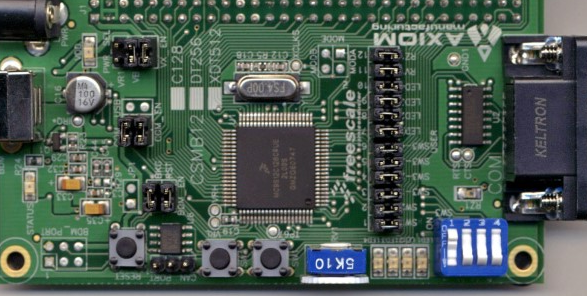
\includegraphics[scale=0.5]{system_setup.png}

        \textbf{System Setup} \\
        NOTE: No hardware other than standard MC9S12C128 module. \\
        Image credit: axman.com/content/csmb-12c128-low-cost-demo-board-freescale-mc9s12c128
    \end{center}

    \begin{center}
        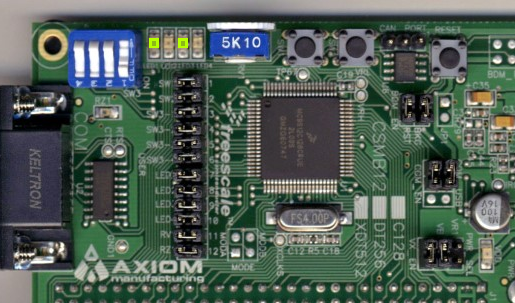
\includegraphics[scale=0.5]{action_shot.png}

        \textbf{Action Shot} \\
        NOTE: No hardware other than standard MC9S12C128 module. \\
        Image credit: axman.com/content/csmb-12c128-low-cost-demo-board-freescale-mc9s12c128
    \end{center}

%-------------------------------------------------------

\sectPart{Public Project Photos}

    \begin{center}
        Our project logo:

        
\includegraphics[scale=0.5]{../../logo.png}

        Our names may be associated with this image.        
    \end{center}

%=======================================================

\end{document}
